\documentclass[parskip=full]{scrartcl}

\usepackage[utf8]{inputenc} % use utf8 file encoding for TeX sources
\usepackage[T1]{fontenc} % avoid garbled Unicode text in pdf
\usepackage[german]{babel} % german hyphenation, quotes, etc
\usepackage{hyperref} % detailed hyperlink/pdf configuration
\hypersetup{ % ‘texdoc hyperref‘ for options
pdftitle={Lamb.da - Das Spiel}
}
\usepackage{csquotes} % provides \enquote{} macro for "quotes"
\usepackage{graphicx}
\usepackage{float}
\usepackage{geometry}
\usepackage{enumerate}

\begin{document}

\title{Lamb.da - Das Spiel}
%\date{October 12, 123}
\author{Name, Name, Name}
\maketitle

\input{./sections/1_introduction.tex}
\input{./sections/2_game_structure.tex}
\input{./sections/3_target_definition.tex}
\input{./sections/4_product_application.tex}
\input{./sections/5_product_environment.tex}
\input{./sections/6_functional_requirements.tex}
\input{./sections/7_product_data.tex}
\input{./sections/8_non_functional_requirements.tex}
\input{./sections/9_use_cases.tex}
\section{Testfälle}
% TODO T Nummern anpassen


\subsection{Globale Testfälle}
Folgende Funktionssequenzen sind zu überprüfen:

\begin{itemize}
\item /T110/ Erstmaliges Starten des Programms
\begin{itemize}
\item Während das Programm sich im Ladebildschirm befindet, werden dem Spieler Comic-artige Sprechblasen mit lustigen und interessanten Texten angezeigt.
\item Der Nutzer startet das Programm und befindet sich im Sprachauswahlmenü $($Abb. \ref{fig:Sprachauswahlmenu}$)$. Mit den Sprachauswahl-Buttons $($S2$)$ wählt er die Sprache Deutsch aus.
\item Durch Drücken des Weiter-Buttons $($B1$)$ wechselt das Programm zum Namenswahlmenü $($Abb. \ref{fig:Namenswahlmenu}$)$. Hier wird der Spieler nach seinem Namen gefragt, den er in der Namenseingabe-Textbox eingibt.
\item Durch Drücken des  Weiter-Buttons $($B1$)$ wechselt das Programm zum Avatarauswahlmenü $($Abb. \ref{fig:Avatarauswahlmenu}$)$.
 Mit den Knöpfen A1 und A2 wählt er den gewünschten Avatar aus.
\item Durch Drücken des Weiter-Buttons $($B1$)$ erscheint der Begrüßungsbildschirm $($Abb. \ref{fig:Begrussungsbildschirm}$)$ mit Name und Avatar des Spielers.
\item Nach 3 Sekunden wechselt das Programm automatisch zum Hauptmenü $($Abb. \ref{fig:Hauptmenu}$)$.
\end{itemize}

\item /T120/ Starten des Programms, nachdem mindestens ein Profil bereits erstellt wurde
\begin{itemize}
\item Der Nutzer startet das Programm und befindet sich im Profilauswahlmenü $($Abb. \ref{fig:Profilauswahlmenu}$)$. Hier wählt er durch Drücken des Name-Button $($P1$)$, welcher mit seinem Namen beschriftet ist, sein Profil aus.
\item Es erscheint der Begrüßungsbildschirm $($Abb. \ref{fig:Begrussungsbildschirm}$)$ mit Name und Avatar des Spielers.
\item Nach 3 Sekunden wechselt das Programm automatisch zum Hauptmenü $($Abb. \ref{fig:Hauptmenu}$)$.
\end{itemize}

\item /T130/ Profildaten ändern
\begin{itemize}
\item Der Nutzer befindet sich im Profilauswahlmenü $($Abb. \ref{fig:Profilauswahlmenu}$)$.
\item Durch Drücken des Konfigurations-Buttons $($P2$)$ öffnet sich ein Dialog-Fenster, in dem der Nutzer die Option "`Profil editieren"' wählt. Das Programm wechselt zum Sprachauswahlmenü $($Abb. \ref{fig:Sprachauswahlmenu}$)$. 
\item Wie in /T110/ beschrieben gibt der Nutzer nacheinander Sprache, Namen und Avatar ein.
\item Nach Drücken des Bestätigungs-Buttons $($B3$)$ im Menü Avatarauswahlmenü $($Abb. \ref{fig:Avatarauswahlmenu}$)$ wechselt das Programm zurück in das Profilauswahlmenü $($Abb. \ref{fig:Profilauswahlmenu}$)$.
\end{itemize}

\item /T140/ Profil löschen
\begin{itemize}
\item Der Nutzer befindet sich im Profilauswahlmenü $($Abb. \ref{fig:Profilauswahlmenu}$)$.
\item Durch Drücken des Konfigurations-Buttons $($P2$)$ öffnet sich ein Dialog-Fenster, in dem der Nutzer die Option "`Profil löschen"' wählt.
\item In einem weiteren Dialog-Fenster bestätigt der Spieler seine Aktion.
\item Das Programm wechselt zurück in das Profilauswahlmenü $($Abb. \ref{fig:Profilauswahlmenu}$)$. Da das Profil jetzt gelöscht ist, erscheint es hier nicht mehr zur Auswahl.
\end{itemize}

\item /T150/ Einen Term im Editor-Modus bearbeiten
\begin{itemize}
\item Der Nutzer hat ein Level gestartet und befindet sich jetzt im Editor-Modus.
% Knops "Hinweis"
\item Durch Drücken des Knopfes TODO öffnet sich ein Popupfenster, in welchem dem Spieler ein Hinweis zur Lösung des aktuellen Levels gegeben wird.
\item Durch die Drag\&Drop Geste fügt er nacheinander sowohl ein weißes Lamm als auch ein weißer Edelstein zum aktuellen Term hinzu.
\item Durch Drücken des Lamms öffnet sich ein Kontextmenü, in dem der Spieler eine Farbe auswählen kann. Nach Drücken der gewünschten Option wechselt das Lamm seine Farbe.
\item Durch die Drag\&Drop Geste zum Werkzeugmenü entfernt der Spieler einen Edelstein aus dem Term.
\item Der Spieler versucht ein durch das Level bereits vorgegebenes Lamm durch die Drag\&Drop Geste zu verschieben, das Programm unterdrückt dies aber.
% Knopf "Play"
\item Der Term ist jetzt gültig und der Spieler drüct den Knopf TODO. Das Programm wechselt zum Reduktions-Modus.
\end{itemize}

\item /T150/ Einen Term im Reduktions-Modus konvertieren
\begin{itemize}
% Knopf "Play"
\item Der Nutzer hat nach Bearbeiten eines Terms im Editor-Modus den Knopf TODO betätigt und befindet sich jetzt im Reduktions-Modus.
% Knopf "Step forward"
\item Durch Drücken des Knopfes TODO wird der Term um einen Schritt reduziert.
% Knopf "Step backward"
\item Durch Drücken des Knopfes TODO wird der Term auf den Zustand vor dem letzten Schritt zurückgesetzt.
% Knopf "Play" "Pause"
\item Durch Drücken des Knopfes TODO werden automatisch einzelne Reduktionen nacheinander ausgeführt. Nach 3 Schritten drückt der Spieler den Knopf TODO und die Ausführung pausiert.
% Knopf "Step forward"
\item Durch Drücken des Knopfes TODO wird der Term um einen Schritt reduziert. Der Term ist jetzt minimal und gleich dem gewünschten Term, der durch das Level vorgegeben ist.
\item Ein Popup-Fenster wird geöffnet, in dem der Spieler darüber informiert wird, dass er das Level abgeschlossen hat.
\end{itemize}

\item /T160/ Level auswählen
\begin{itemize}
\item Der Nutzer befindet sich im Hauptmenü $($Abb. \ref{fig:Hauptmenu}$)$ und drückt den Level-Button $($H2$)$. Das Programm wechselt zum Levelauswahlmenü $($Abb. \ref{fig:Levelauswahlmenu}$)$.
\item Einige Level sind bereits abgeschlossen und durch einen Haken markiert, ein Level ist freigeschaltet und die restlichen Level nicht freigeschaltet und deshalb durch ein Schloss markiert. Level mit demselben Schwierigkeitsgrad sind hier farblich gleich gekennzeichnet.
\item Der Spieler wählt das erste Level durch Drücken des Levelstart-Buttons $($L1$)$ aus und das Programm wechselt in den Editor-Modus zur Bearbeitung dieses Levels.
\end{itemize}

\item /T170/ Das Einkaufsmenü benutzen
\begin{itemize}
\item Der Spieler besitzt durch Abschluss mehrerer Level eine Anzahl an Münzen. Bisher hat er noch keine Elemente im Shop gekauft.
\item Das Programm befindet sich im Hauptmenü $($Abb. \ref{fig:Hauptmenu}$)$. Durch Drücken des Einkaufs-Button $($H6$)$ wechselt es zum Einkaufsmenü $($Abb. \ref{fig:Einkaufsmenu}$)$.
\item Hier wählt der Spieler das Musik-Dropdownmenü $($E1$)$ aus. Es erscheinen mehrere zum Kauf verfügbare Objekte $($Abb. \ref{fig:Einkaufsmenu_Dropdown}$)$.
\item Der Spieler wählt den ersten Sound aus und wird darauf durch ein Dialog-Fenster zur Bestätigung des Kaufs gebeten.
\item Nach der Bestätigung wird der Sound freigeschaltet und automatisch aktiviert.
\item Durch Wiederholen dieser Schritte kauft er auch den zweiten verfügbaren Sound. Dieser wird automatisch aktiviert.
\item Der Spieler aktiviert nun wieder den ersten Sound, indem er auf das zweite Element drückt. Das aktivierte erste Element wird durch einen Haken gekennzeichnet, der Haken beim deaktivierten zweiten Element wird entfernt.
\end{itemize}

\item /T180/ Optionen auswählen
\begin{itemize}
\item Das Programm befindet sich im Hauptmenü $($Abb. \ref{fig:Hauptmenu}$)$. Durch Drücken der Stumm-Checkbox $($H5$)$ wird die Hintergrundmusik deaktiviert.
\item Durch Drücken des Optionen-Buttons $($H4$)$ wechselt das Programm in das Optionsmenü $($Abb. \ref{fig:Optionsmenu}$)$. Hier aktiviert der Spieler durch Drücken der Lehrermodus-Checkbox $($O1$)$ den Lehrermodus und durch Drücken der Farbenblindenmodus-Checkbox $($O2$)$ den Farbenblindenmodus.
\item Durch Verschieben des Geräusche-Sliders $($O4$)$ passt der Spieler die Geräuschelautstärke und durch Verschieben des Musik-Sliders $($O5$)$ die Musiklautstärke an.
\item Durch Drücken des Zurück-Buttons $($B2$)$ wechselt das Programm zurück in das Hauptmenü $($Abb. \ref{fig:Hauptmenu}$)$.
\end{itemize}

\item /T190/ Benutzerstatistik ansehen
\begin{itemize}
\item Das Programm befindet sich im Hauptmenü $($Abb. \ref{fig:Hauptmenu}$)$. Durch Drücken des Erfolge-Buttons $($H3$)$ wechselt das Programm in das Erfolgsmenü $($Abb. \ref{fig:Erfolgsmenu}$)$. Hier kann der Spieler seine abgeschlossenen Erfolge einsehen.
\item Durch Drücken des Zurück-Buttons $($B1$)$ wechselt das Programm zurück in das Hauptmenü $($Abb. \ref{fig:Hauptmenu}$)$.
\item Durch Drücken des Optionen-Buttons $($H4$)$ wechselt das Programm in das Optionsmenü $($Abb. \ref{fig:Optionsmenu}$)$.
\item Durch Drücken des Statistik-Buttons $($O3$)$ wechselt das Programm in das Statistikmenü $($Abb. \ref{fig:Statistikmenu}$)$. Hier kann der Spieler Statistiken zu seinem Spielverhalten einsehen.
\item Durch Drücken des Zurück-Buttons $($B2$)$ wechselt das Programm zurück in das Optionsmenü $($Abb. \ref{fig:Optionsmenu}$)$.
\item Durch Drücken des Zurück-Buttons $($B2$)$ wechselt das Programm zurück in das Hauptmenü $($Abb. \ref{fig:Hauptmenu}$)$.
\end{itemize}

\end{itemize}

\subsection{Datenkonsistenzen}
Folgende Datenkonsistenzen sind zu überprüfen:

\begin{itemize}
\item /T210/ Ein Profil ist eindeutig durch den Namen gekennzeichnet. Es kann nicht mehrere Profile mit demselben Namen geben.
\end{itemize}

\section{Systemmodelle}
% TODO T Nummern anpassen

\subsection{Objektmodelle}
% UML Klassendiagramme

\begin{figure}[H]
\centering
\includegraphics[scale=0.5]{../system_models/object_models/lambda_calculus.pdf}
\caption{UML Klassendiagramm zum Lambda-Kalkül}
\end{figure}

\subsection{Dynamische Modelle}
% UML Zustandsautomat, Sequenzdiagramm

%\newgeometry{left=40pt}
\begin{figure}[H]
\centering
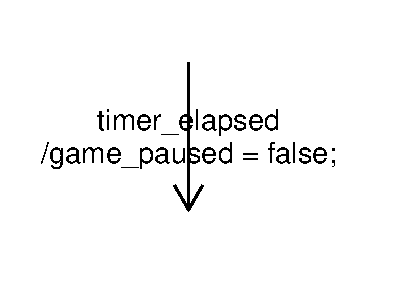
\includegraphics[scale=0.4]{../system_models/dynamic_models/menu_state_machine.pdf}
\caption{Zustandsautomat zur Menübedienung}
\end{figure}
%\restoregeometry

\begin{figure}[H]
\centering
\includegraphics[scale=0.55]{../system_models/dynamic_models/game_level_state_machine.pdf}
\caption{Zustandsautomat zum Ablauf eines Levels}
\end{figure}

\begin{figure}[H]
\centering
\includegraphics[scale=0.55]{../system_models/dynamic_models/reduction_mode_state_machine.pdf}
\caption{Zustandsautomat zur Funktion des Reduktions-Modus}
\end{figure}

\subsection{Benutzerschnittstelle}
%../GUI-Entwurf/_jpeg_numeration/registration1.gpej
%1-pflichtenheft/
\newcounter{B.SS}
\begin{figure}[H]

\centering
\refstepcounter{B.SS}\label{fig:Sprachauswahl}
\includegraphics[scale=0.55]{../GUI-Entwurf/_jpeg_numeration/registration1.jpg}

\caption{Sprachauswahl}


\end{figure}

\begin{figure}[H]
\centering
\refstepcounter{B.SS}\label{fig:Nameneingabe} 
\includegraphics[scale=0.55]
{../GUI-Entwurf/_jpeg_numeration/registration2.jpg}
\caption{Nameneingabe}
\end{figure}

\begin{figure}[H]
\centering
\refstepcounter{B.SS}\label{fig:Awatarauswahl}
\includegraphics[scale=0.55]{../GUI-Entwurf/_jpeg_numeration/registration3.jpg}
\caption{Awatarwahl}
\end{figure}

\begin{figure}[H]
\centering
\refstepcounter{B.SS}\label{fig:Profilauswahl}
\includegraphics[scale=0.55]{../GUI-Entwurf/_jpeg_numeration/choose_profile.jpg}
\caption{Profilauswahl}
\end{figure}

\begin{figure}[H]
\centering
\refstepcounter{B.SS}\label{fig:Welcome}
\includegraphics[scale=0.55]{../GUI-Entwurf/_jpeg_numeration/welcome.jpg}
\caption{Begrüssungsbildschirm}
\end{figure}

\begin{figure}[H]
\centering
\refstepcounter{B.SS}\label{fig:Hauptmenu}
\includegraphics[scale=0.55]{../GUI-Entwurf/_jpeg_numeration/main_manu.jpg}
\caption{Hauptmenu}
\end{figure}

\begin{figure}[H]
\centering
\refstepcounter{B.SS}\label{fig:Einstellungen}
\includegraphics[scale=0.55]{../GUI-Entwurf/_jpeg_numeration/settings.jpg}
\caption{Einstellungen}
\end{figure}

\begin{figure}[H]
\centering
\refstepcounter{B.SS}\label{fig:Status}
\includegraphics[scale=0.55]{../GUI-Entwurf/_jpeg_numeration/stat.jpg}
\caption{Status}
\end{figure}

\begin{figure}[H]
\centering
\refstepcounter{B.SS}\label{fig:achievments}
\includegraphics[scale=0.55]{../GUI-Entwurf/_jpeg_numeration/achievments.jpg}
\caption{Achievements}
\end{figure}

\begin{figure}[H]
\centering
\refstepcounter{B.SS}\label{fig:level}
\includegraphics[scale=0.55]{../GUI-Entwurf/_jpeg_numeration/level.jpg}
\caption{Levels}
\end{figure}

\begin{figure}[H]
\refstepcounter{B.SS}\label{fig:shop}
\centering
\includegraphics[scale=0.55]{../GUI-Entwurf/_jpeg_numeration/shop.jpg}
\caption{Shop}
\end{figure}

\begin{figure}[H]
\refstepcounter{B.SS}\label{fig:shop_popup}
\centering
\includegraphics[scale=0.55]{../GUI-Entwurf/_jpeg_numeration/shop_popup.jpg}
\caption{shoppopup}
\end{figure}







\section{Glossar}

\begin{description}
	\item[Achievement] \hfill \\
	Errungenschaft/Erfolg. Bezeichnet eine Auszeichnung für eine bestimmte Leistung.\\
	Kann im Spiel gewonnen werden.\\
	Beispiel: "Lambda für Anfänger" - Du hast das Tutorial erfolgreich abgeschlossen
	
	\item[Android] \hfill \\
	Betriebssystem und Softwareplattform hauptsächlich für mobile Geräte. Das Spiel/Produkt wird in erster Linie 
	für Android entwickelt.
	
	\item[App] \hfill \\
	Kurz für Application oder Applikation und bezeichnet Anwendungssoftware. Im Deutschen meistens jene von mobilen Geräten.
	
	\item[Avatar] \hfill \\
	Im Profil des Benutzers ist der Avatar, ein Bild, aus einer vorgefertigten Sammlung wählbar.
	Der Avatar soll, mit dem Profilnamen, den Nutzer repräsentiert und ist rein kosmetisch.
	Ziel ist dem Spieler die Möglichkeit zu geben sein Profil persönlicher gestalten.
	
	\item[Beta-Konversion] \hfill \\
	Stellt im Lambda-Kalkül das Konzept der Funktionsanwendung dar.
	
	\item[Checkbox] \hfill \\
	Ein Element grafischer Benutzeroberflächen. Wird meist als Kästchen dargestellt, das mit einem Klick aktiviert (abgehakt) oder
	wieder deaktiviert wird. Zum Beispiel um die Musik in einem Spiel an oder aus zu stellen.
	
	\item[Drag\&Drop-Geste] \hfill \\
	Der Benutzer klickt ein Objekt auf dem Bildschirm. Solange er nicht loslässt, "zieht" er das Objekt, wodurch
	es sich typischerweise mit seinem Finger mitbewegt. Lässt er los, lässt er das Objekt wieder "fallen", wodurch
	es an seinem neuen Platz abgelegt wird.
	
	\item[Editor] \hfill \\
	%TODO 
	
	\item[Lambda-Kalkül] \hfill \\
	Das Lambda-Kalkül ist eine formale Sprache, die zur Untersuchung von mathematischen Funktionen entwickelt wurde.
	Die Grundlagen des Lambda-Kalküls zu erlernen ist das Ziel des Produkts.
	
	\item[Level] \hfill \\
	Hier bezeichnet ein Level ein abgeschlossenen Teil des Spiels. Der Spieler betritt/startet das Level. Ihm wird eine Aufgabe,
	wie zum Beispiel ein Rätsel gestellt. Nach dem Abschließen der Aufgabe verlässt der Spieler das Level wieder.
	
	\item[Modus] \hfill \\
	%TODO
	
	\item[Münzen] \hfill \\
	Virtuelle Währung des Spiels. Sie kann zum Beispiel durch erfolgreiches Abschließen eines Levels verdient werden.
	Gewonnene Münzen können im Spiel dann wiederum ausgegeben werden.
	
	\item[Pinch-Geste] \hfill \\
	Durch Berührung zweier Punkte auf dem Bildschirm wird zwischen ihnen ein nicht sichtbares Zentrum erzeugt.
	Bewegt der Benutzer seine Finger näher zum Zentrum oder entfernt er sie weiter davon werden für gewöhnlich
	Aktionen wie die, entsprechend der Bewegung, Vergrößerung oder Verkleinerung von Objekten durchgeführt.
	
	\item[Popup] \hfill \\
	Popups sind kleinere Fenster, die auf dem Bildschirm erscheinen und das Fenster hinter ihnen teilweise verdecken.
	Sie zeigen oft zusätzliche Inhalte an oder suchen Bestätigung für eine Aktion des Nutzers.
	
	\item[Profil] \hfill \\
	Profile machen das Benutzen des Spiels von mehreren Personen möglich. Jeder Benutzer hat ein eigenes Profil,
	dass alle seine Daten (Name, Spielfortschritt usw.) speichert. Der Benutzer wählt beim Start sein Profil aus, wodurch das Spiel,
	wie er es zuvor verlassen hat, geladen wird, obwohl zum Beispiel in der Zwischenzeit ein Zweiter auf einem anderen Profil gespielt hat.
	
	\item[Reduktion] \hfill \\
	Oder Beta-Reduktion. Anderer Name für die Beta-Konversion, falls diese ausschließlich von links nach rechts angewandt wird.
	
	\item[Shop] \hfill \\
	Der Shop ist ein Menü im Spiel, indem die im Spiel existierende Währung der Münzen gegen verschiedenste Dinge eingetauscht werden kann.
	
	\item[Smartphone] \hfill \\
	Ein mobiles Telefon, dass mehr Computer-Funktionalitäten besitzt, als ein herkömmliches Telefon. Häufiges Merkmal ist ein sogenannter
	Touchscreen, der zu einem großen Teil zur Bedienung benutzt wird.
	
	\item[Tablet] \hfill \\
	Es ähnelt einem Smartphone und verwendet häufig auch für Smartphones entwickelte Betriebssysteme. 
	Ein Tablet ist aber normalerweise um ein Vielfaches größer und besitzt dadurch einen größeren Touchscreen.

	\item[Term] \hfill \\
	Mit einem Term wird hier ein Ausdruck im Lambda-Kalkül beschrieben. Das Spiel basiert auf der Idee solche Terme kindgerecht 
	zu visualisieren.
	
	\item[Touchscreen] \hfill \\
	Berührungsempfindlicher Bildschirm. Durch Berührungen und Gesten auf dem Touchscreen kann ein Gerät bedient werden.
	
	\item[Zoom] \hfill \\
	Durch Zoomen scheint Spieler den Bildausschnitt näher zu einem Objekt zu bewegen oder ihn weiter davon zu entfernen.
	Dadurch kann der Nutzer kleine Objekte größer darstellen oder sich bei vielen Objekten einen Überblick "von oben" verschaffen. 
\end{description}


\end{document}